%\clearpage
%\subsection{Control Regions (CRs) definitions}
\label{subsec:cr_selection}

In this analysis, we adopt the conventional approach for background estimation, which combines MC simulations with data-driven methods. MC simulations are used to model SM background processes, while dedicated Control Regions (CRs) are established to adjust the background normalization within the SRs.
This section will detail the definition of CRs tailored to $W$+jets and \ttbar events. Furthermore, we distinguish between CRs for the resolved and merged categories to address potential discrepancies in background modeling across different \pt ranges.

\subsection{$W$+jets Control Region (WCR)}
\label{wcr_definition}

The $W$+jets Control Region (WCR) is defined using mass sidebands relative to the hadronically decaying vector boson. Notably, in the resolved category, distinct sidebands outside the mass windows of both the $W$ and $Z$ bosons are identifiable.
In contrast, in the merged category, the definition becomes more conceptual due to the event selection methodology. The criteria for event selection in the WCR are aligned with those in the SR to ensure analytical consistency:
 
\begin{itemize}
    \item In the resolved category, events must satisfy $50 < m_{jj} < 64$ GeV or $m_{jj} > 106$ GeV, effectively inverting the $m_{jj}$ requirement for the SR.
    \item In the merged category, the criterion is failing the high efficiency WP ($\epsilon=80\%$) of the vector boson tagger.
\end{itemize}

Figure \ref{fig:1lepMVHadResCR} shows the sideband distributions for $m_{jj}$ in the resolved WCR.
Figure \ref{fig:1lepMVHadMerCR} shows the large-R jet mass distributions in the merged control region. Given that the merged CR is defined by the vector boson tagger's $80\%$ working point, the mass distribution encompasses events within both the sidebands and the mass window.

In the resolved category, the ``Loose'' and ``Tight'' regions are defined similarly to those in the resolved SR. The $m_{jjj}$ distributions are shown in Figure~\ref{fig:1lepWCR_mjjj}, where the peak at about $180\,\si{\GeV}$, corresponding to the top quark mass, is observed in the ``Loose'' region. This indicates that the cut at $220\,\si{\GeV}$ was effective in excluding this peak from the ``Tight'' region.

\begin{figure}[ht]
    \centering
    \begin{subfigure}{0.32\textwidth}
        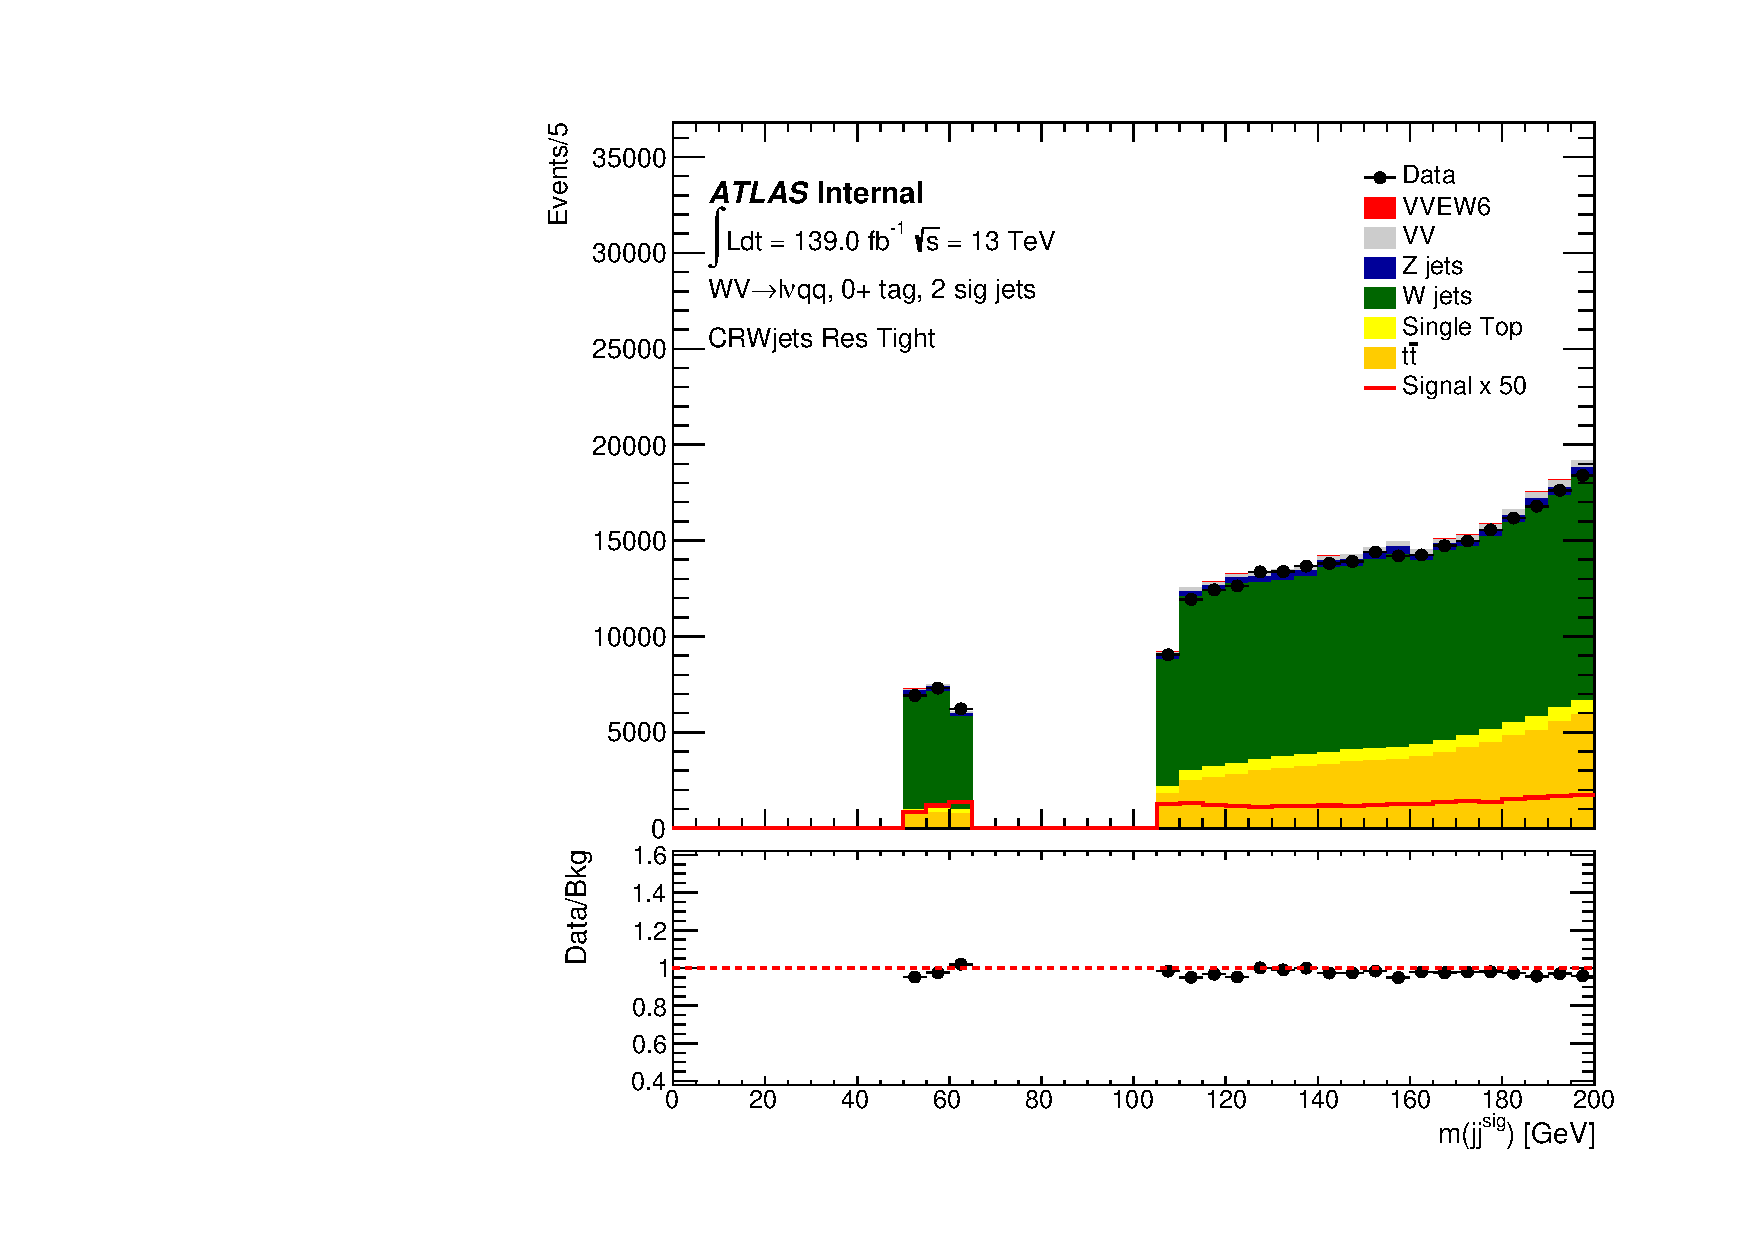
\includegraphics[width=\linewidth]{figures/CRPlots/CRWjets_Res_Tight/stacked_plot_Dijet_m.pdf}
        \caption{$m_{jj}$ plot in the sidebands.\\ \hspace*{1.5cm}Resolved WCR.}
        \label{fig:1lepMVHadResCR}
    \end{subfigure}
    \begin{subfigure}{0.32\textwidth}
        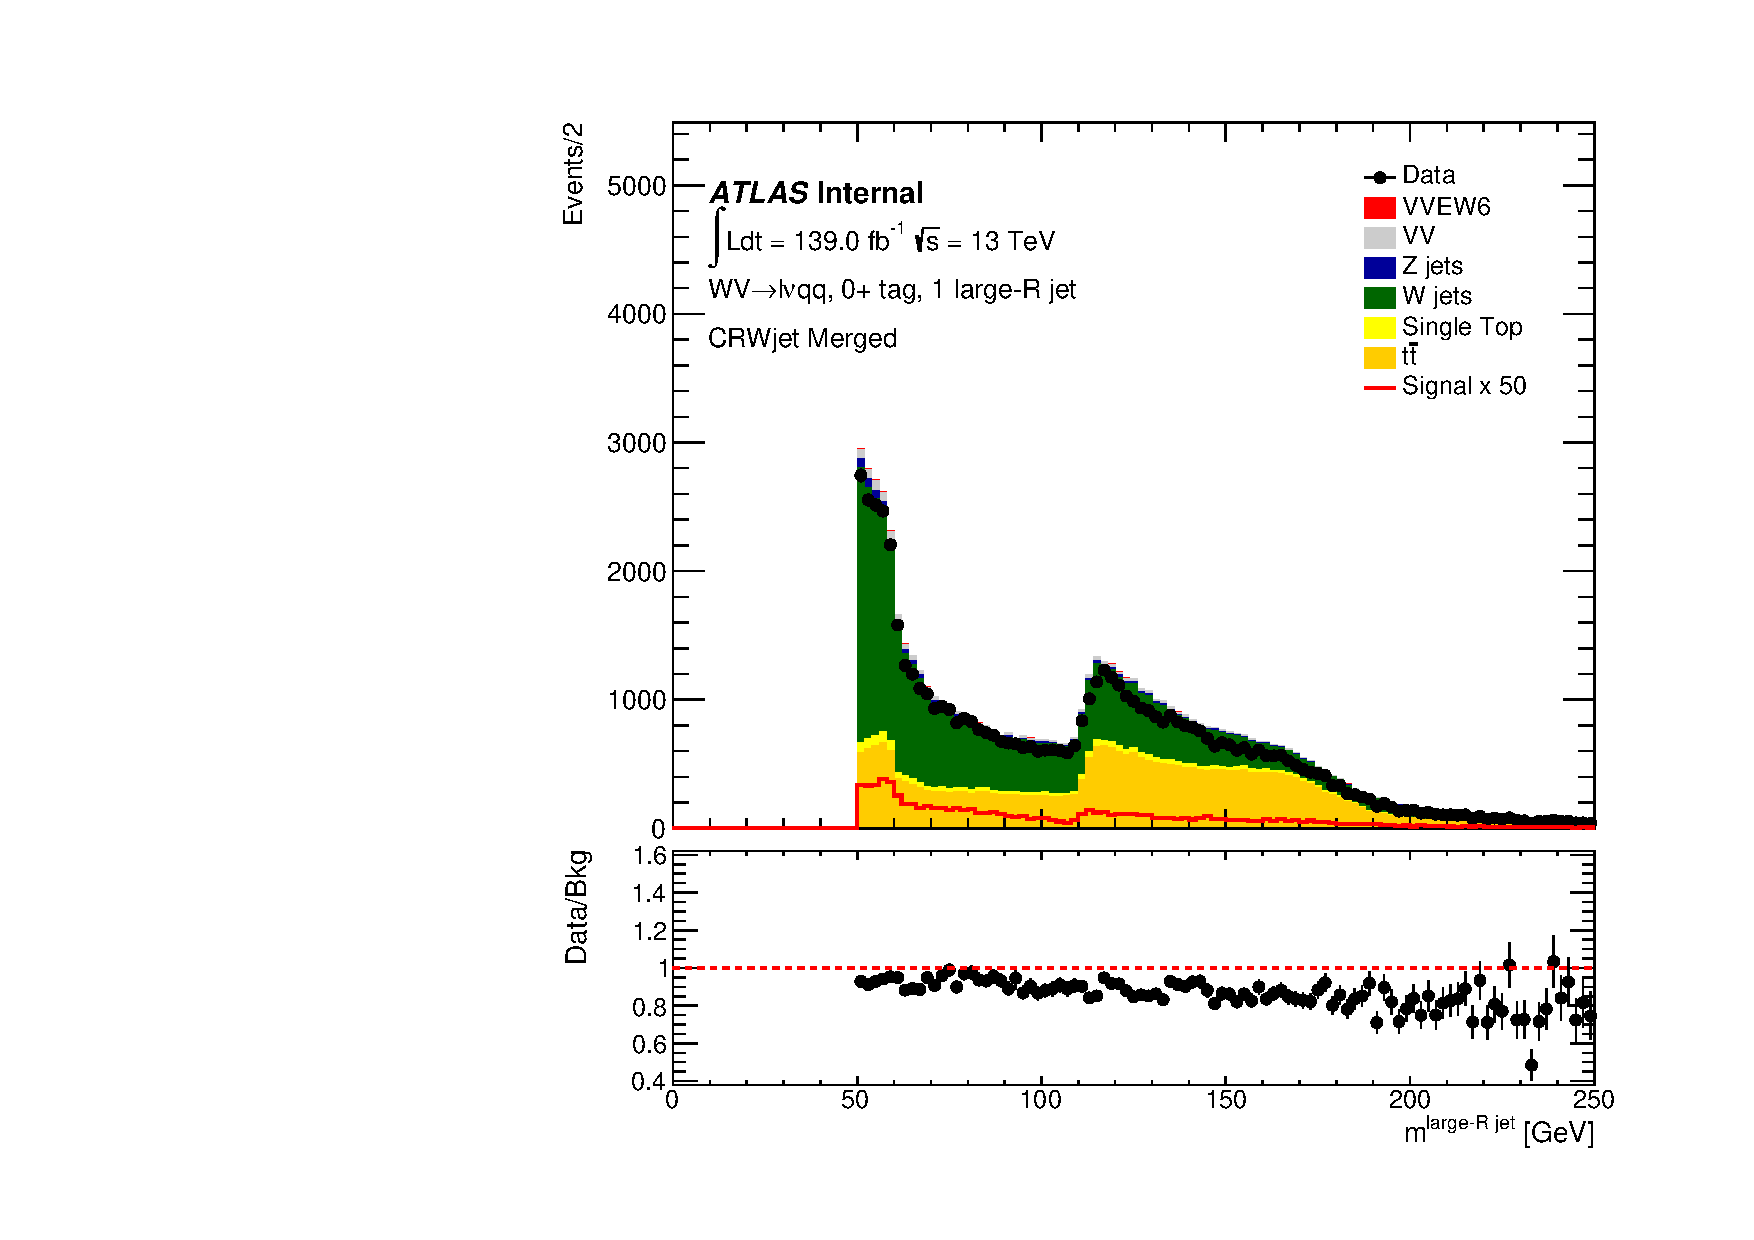
\includegraphics[width=\linewidth]{figures/CRPlots/CRWjets100/stacked_plot_fatJ_m.pdf}
        \caption{$m_{J}$ plot in the ``sidebands.''\\ \hspace*{1.5cm}Merged WCR.}
        \label{fig:1lepMVHadMerCR}
    \end{subfigure}
    \caption{$m_{V_{Had}}$ ($m_{jj}$ or $m_{J}$) plots in the resolved and merged WCRs.}
    \label{fig:1lepMVHad}
\end{figure}

\begin{figure}[ht]
    \centering
    \begin{subfigure}{0.32\textwidth}
        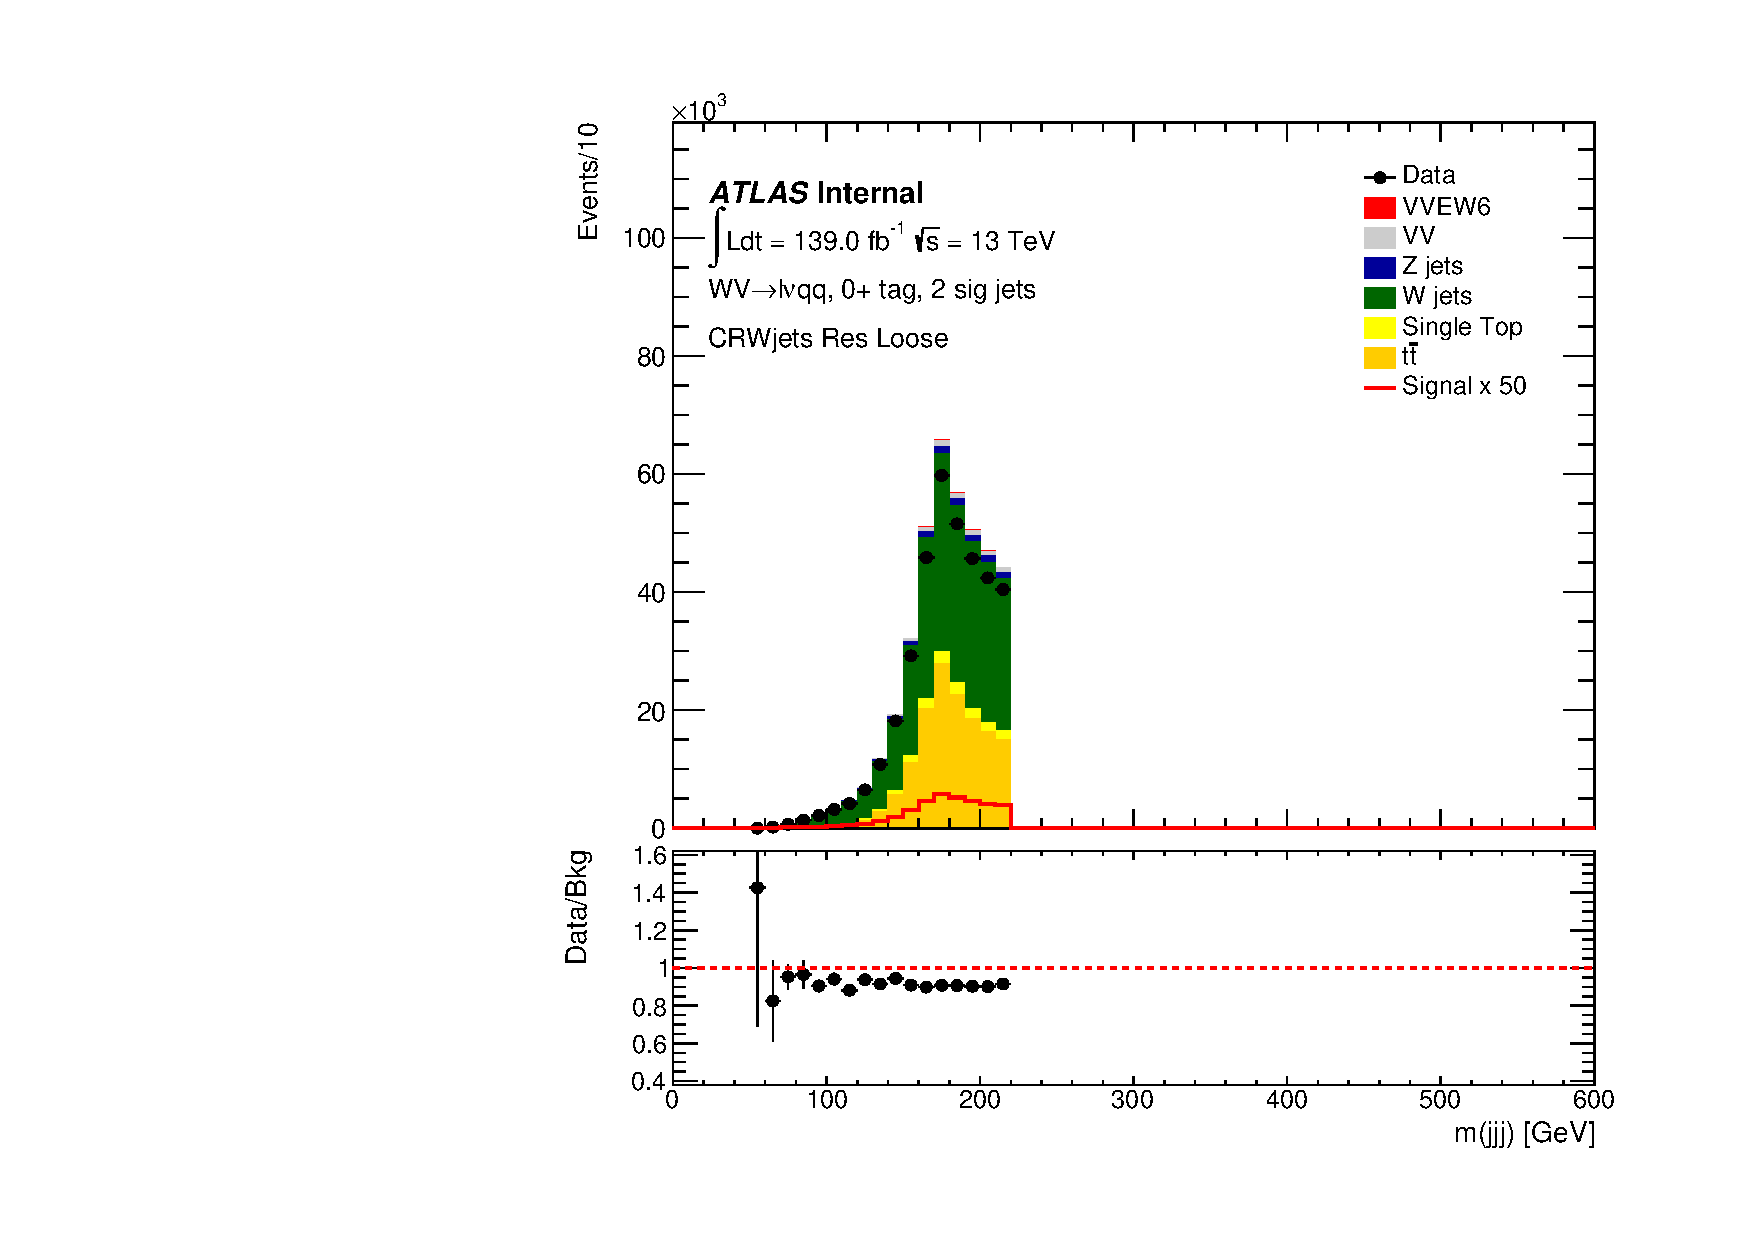
\includegraphics[width=\linewidth]{figures/CRPlots/CRWjets_Res_Loose/stacked_plot_Mjjj.pdf}
        \caption{Resolved ``Loose'' WCR.}
%        \label{fig:1lepMVHadResCR}
    \end{subfigure}
    \begin{subfigure}{0.32\textwidth}
        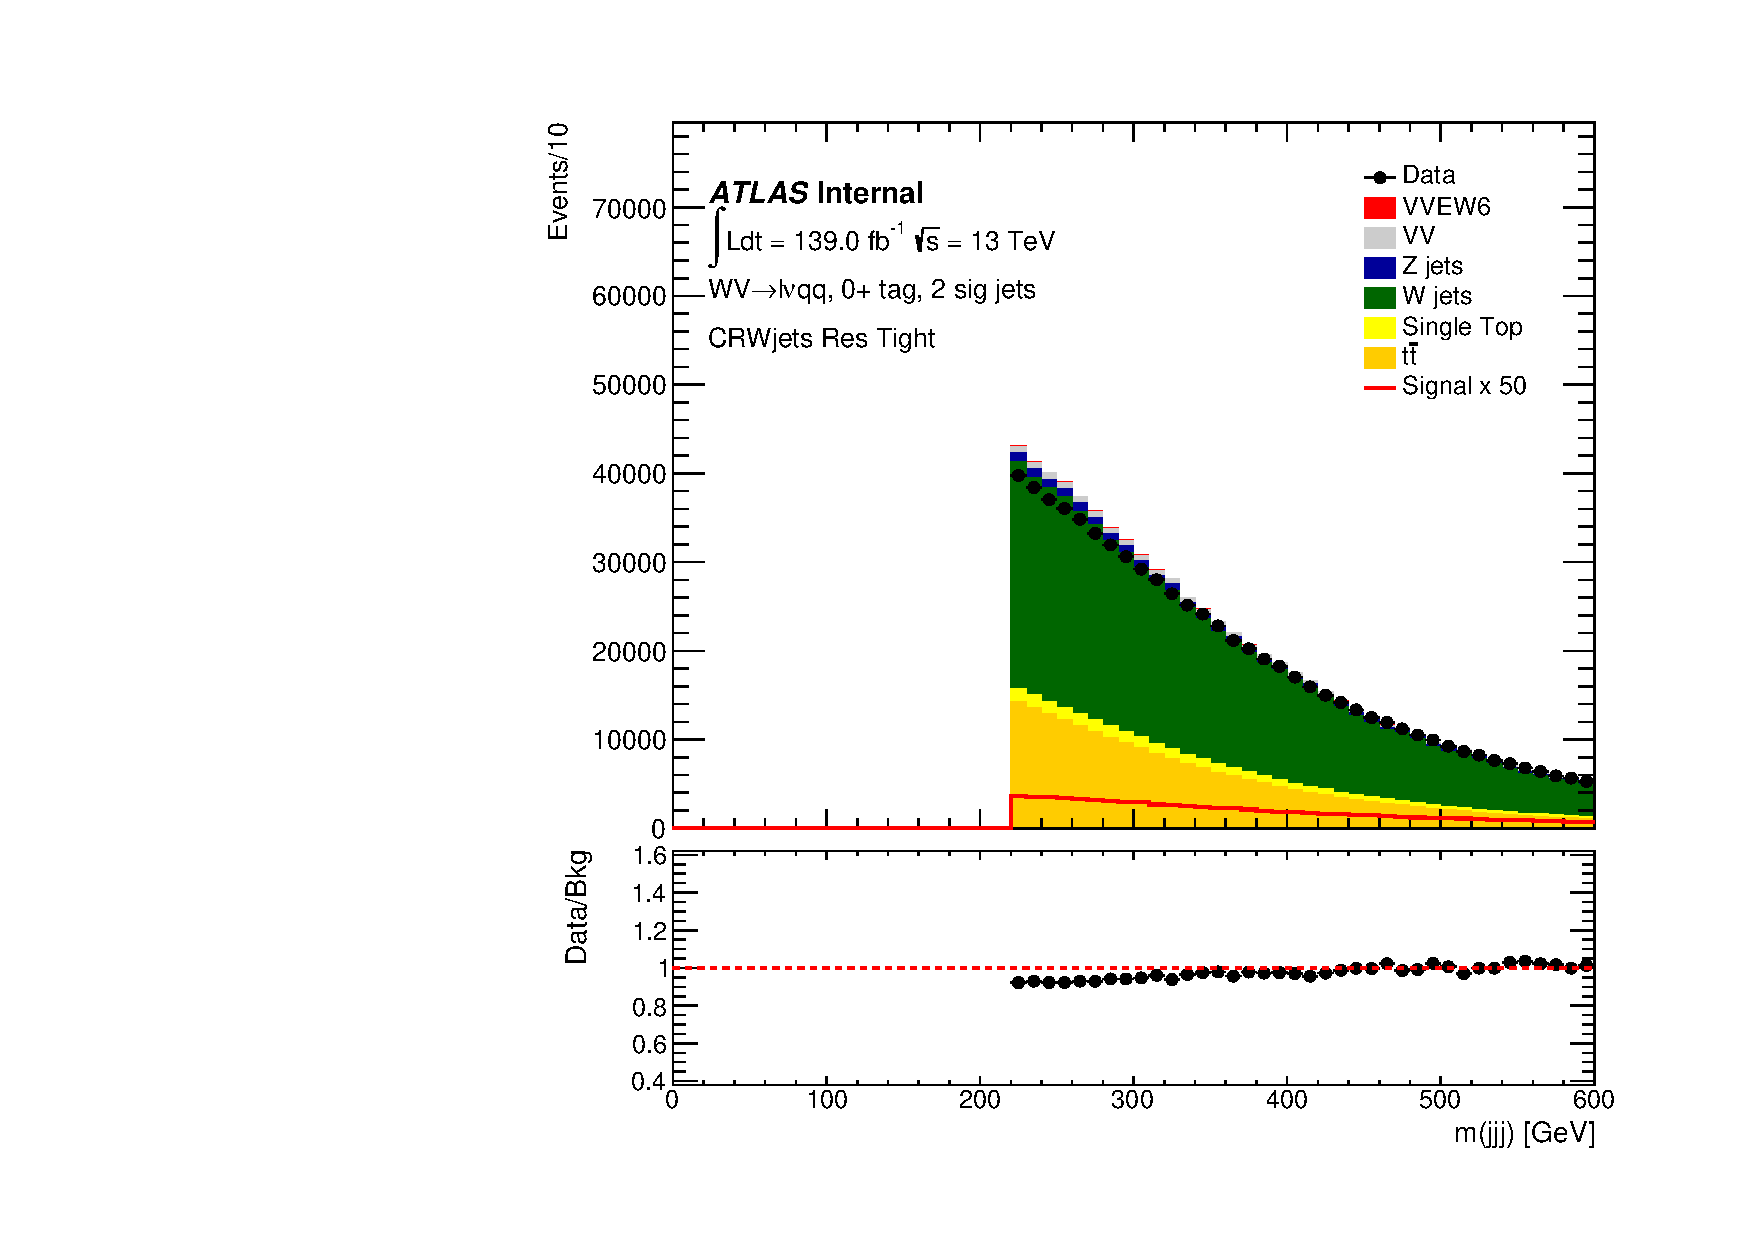
\includegraphics[width=\linewidth]{figures/CRPlots/CRWjets_Res_Tight/stacked_plot_Mjjj.pdf}
	\caption{Resolved ``Tight'' WCR.}
%        \label{fig:1lepMVHadMerCR}
    \end{subfigure}
    \caption{$m_{jjj}$ plots in the ``Loose'' and ``Tight'' WCRs.}
    \label{fig:1lepWCR_mjjj}
\end{figure}


%\clearpage
\subsection{Top Control Region (TCR)}
\label{tcr_definition}

The TCR is established by requiring the presence of at least one $b$-tagged jet, contrary to a $b$-veto in other regions. Figure \ref{fig:1lepNBjetsPresel} displays the $b$-jets multiplicity distributions for both the resolved and merged regimes. 
The defining feature of the TCR, the inclusion of additional $b$-jets, creates orthogonal cuts that align with the mass window phase spaces. 
In the merged regime, the TCR adopts the High Purity (HP) and Low Purity (LP) categorization analogous to the SRs.

\begin{figure}[ht]
    \centering
    \begin{subfigure}{0.32\textwidth}
        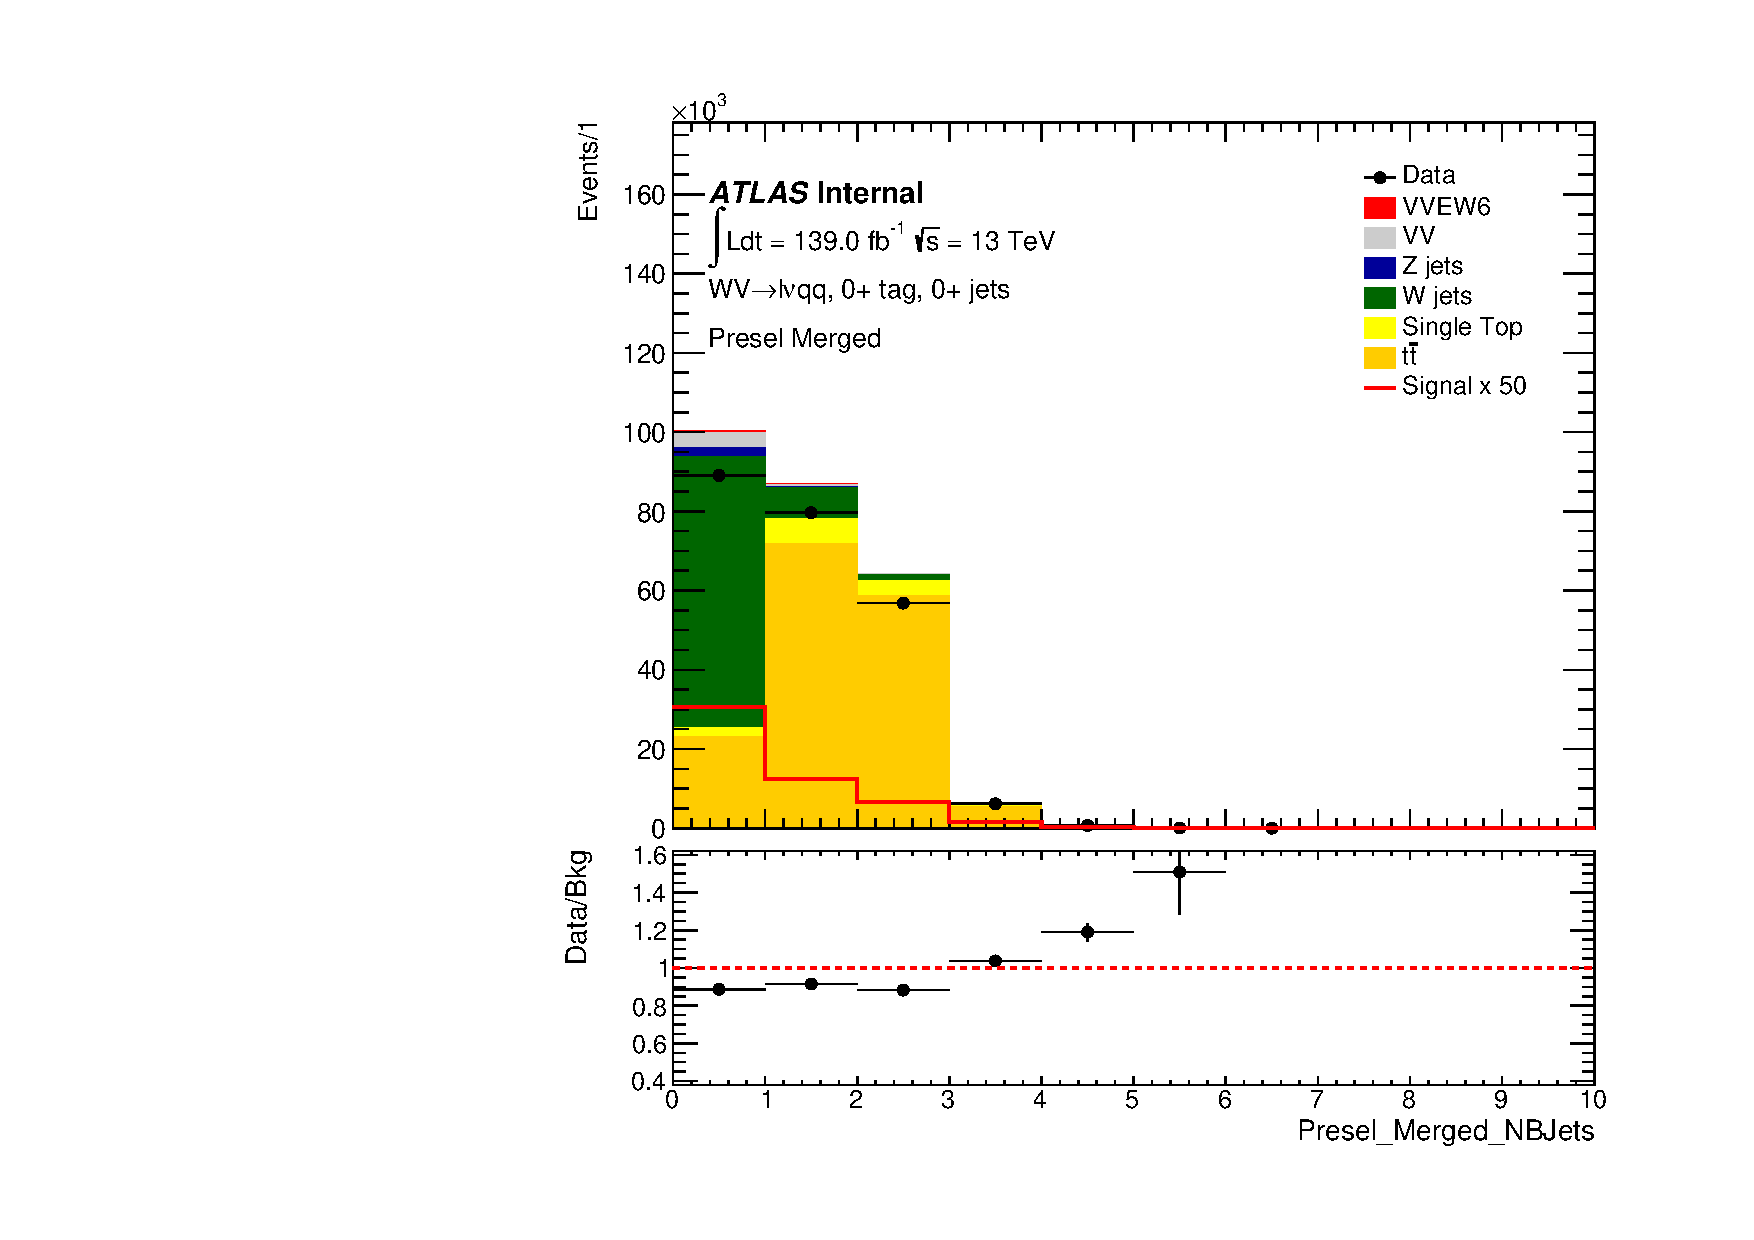
\includegraphics[width=\linewidth]{figures/event_selection/Presel_Merged_NBJets.pdf}
        \caption{After merged preselection}
    \end{subfigure}
    \begin{subfigure}{0.32\textwidth}
        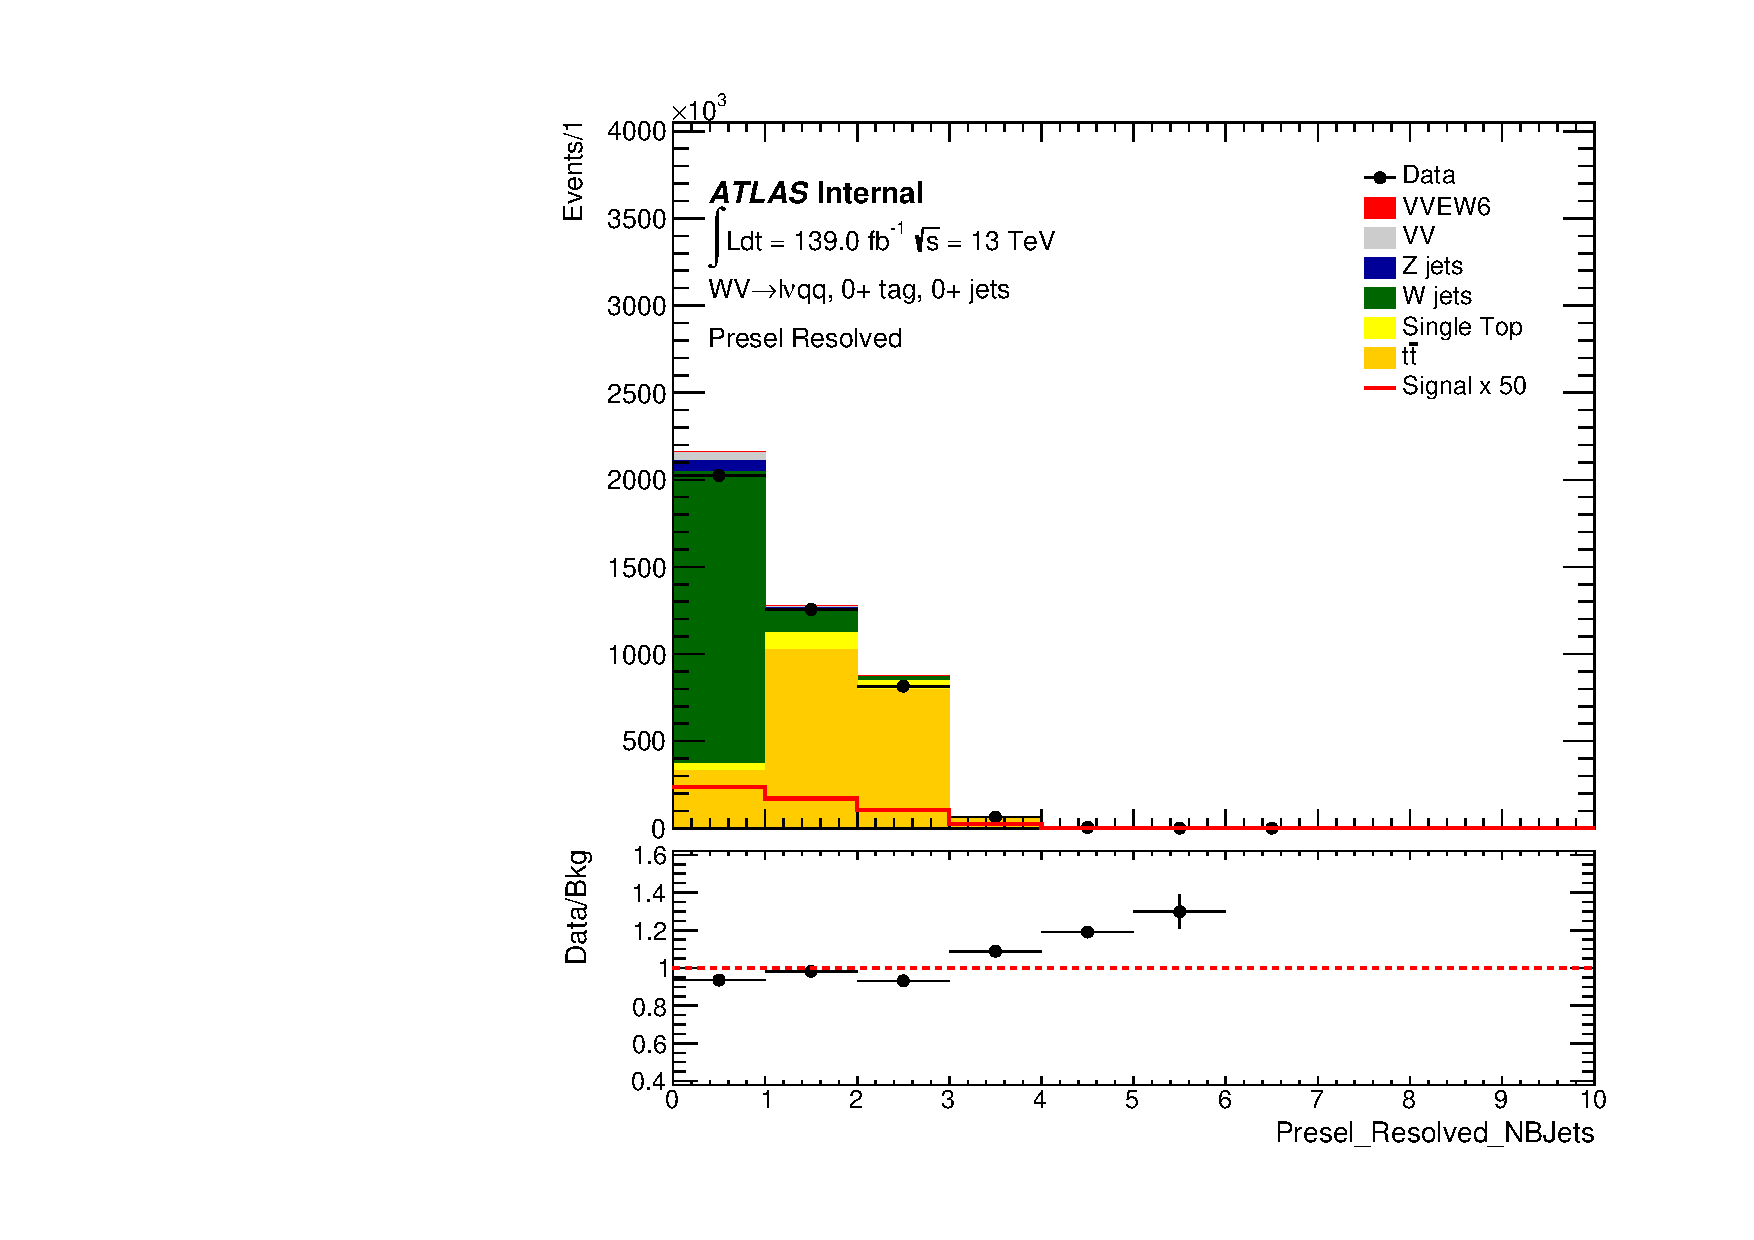
\includegraphics[width=\linewidth]{figures/event_selection/Presel_Resolved_NBJets.pdf}
        \caption{After resolved preselection}
    \end{subfigure}\\
    \begin{subfigure}{0.32\textwidth}
        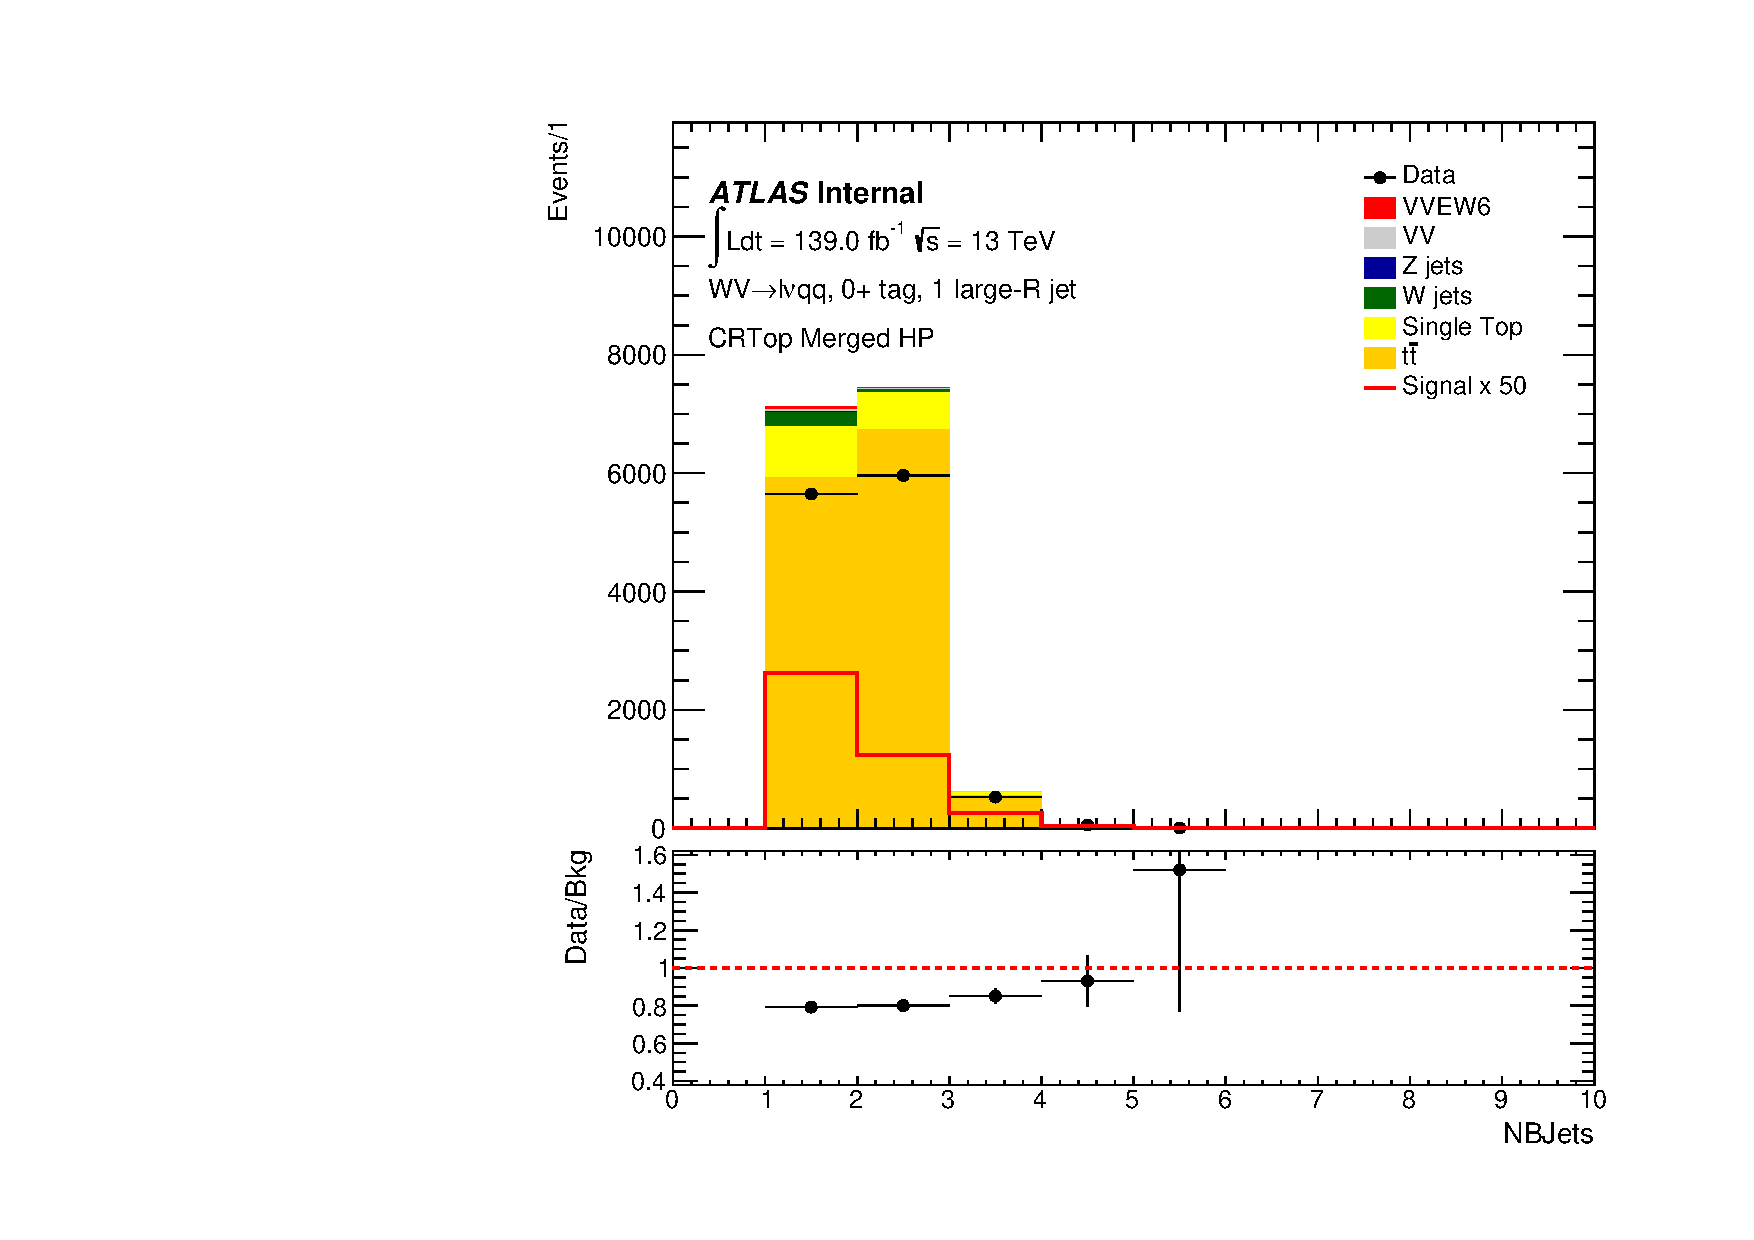
\includegraphics[width=\linewidth]{figures/CRPlots/CRTop_50/stacked_plot_NBJets.pdf}
        \caption{HP TCR}
    \end{subfigure}
    \begin{subfigure}{0.32\textwidth}
        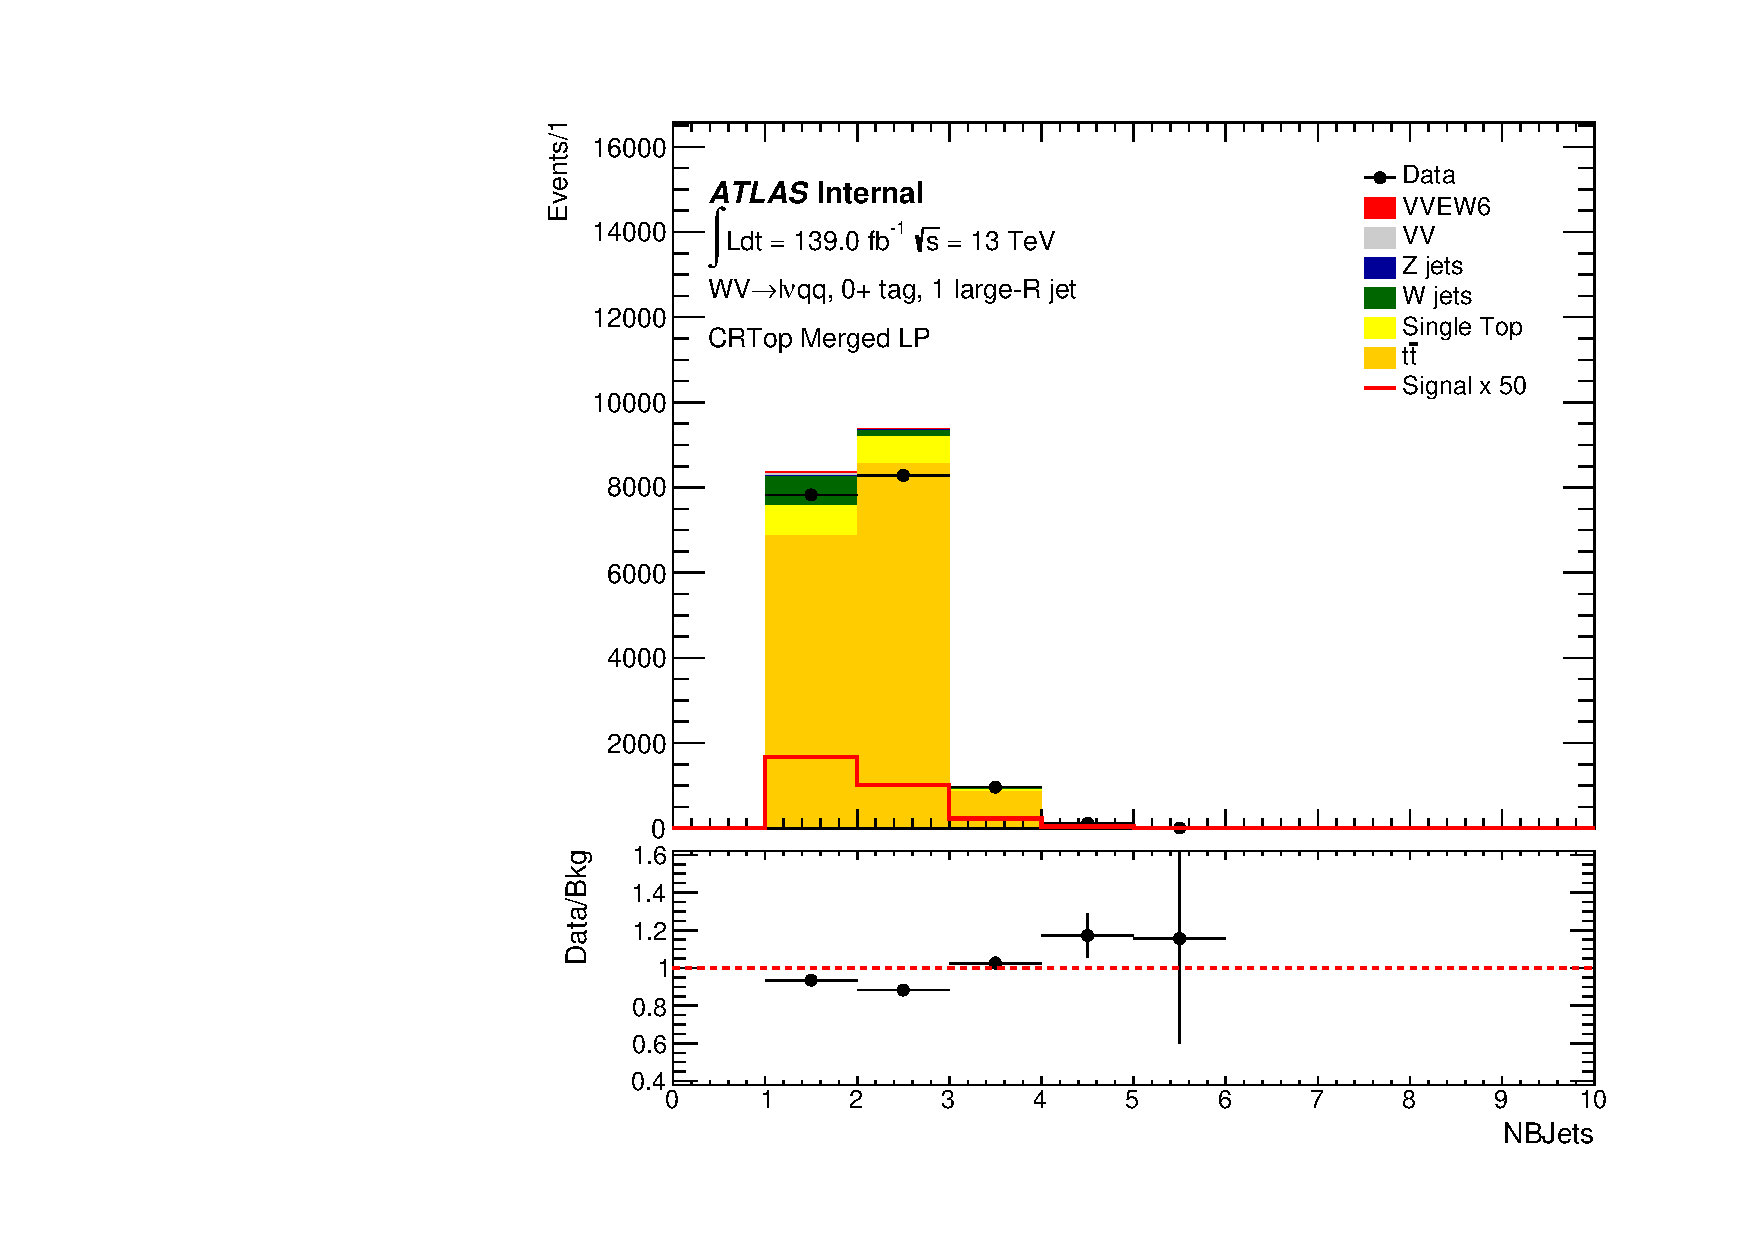
\includegraphics[width=\linewidth]{figures/CRPlots/CRTop_80/stacked_plot_NBJets.pdf}
        \caption{LP TCR}
    \end{subfigure}
    \begin{subfigure}{0.32\textwidth}
        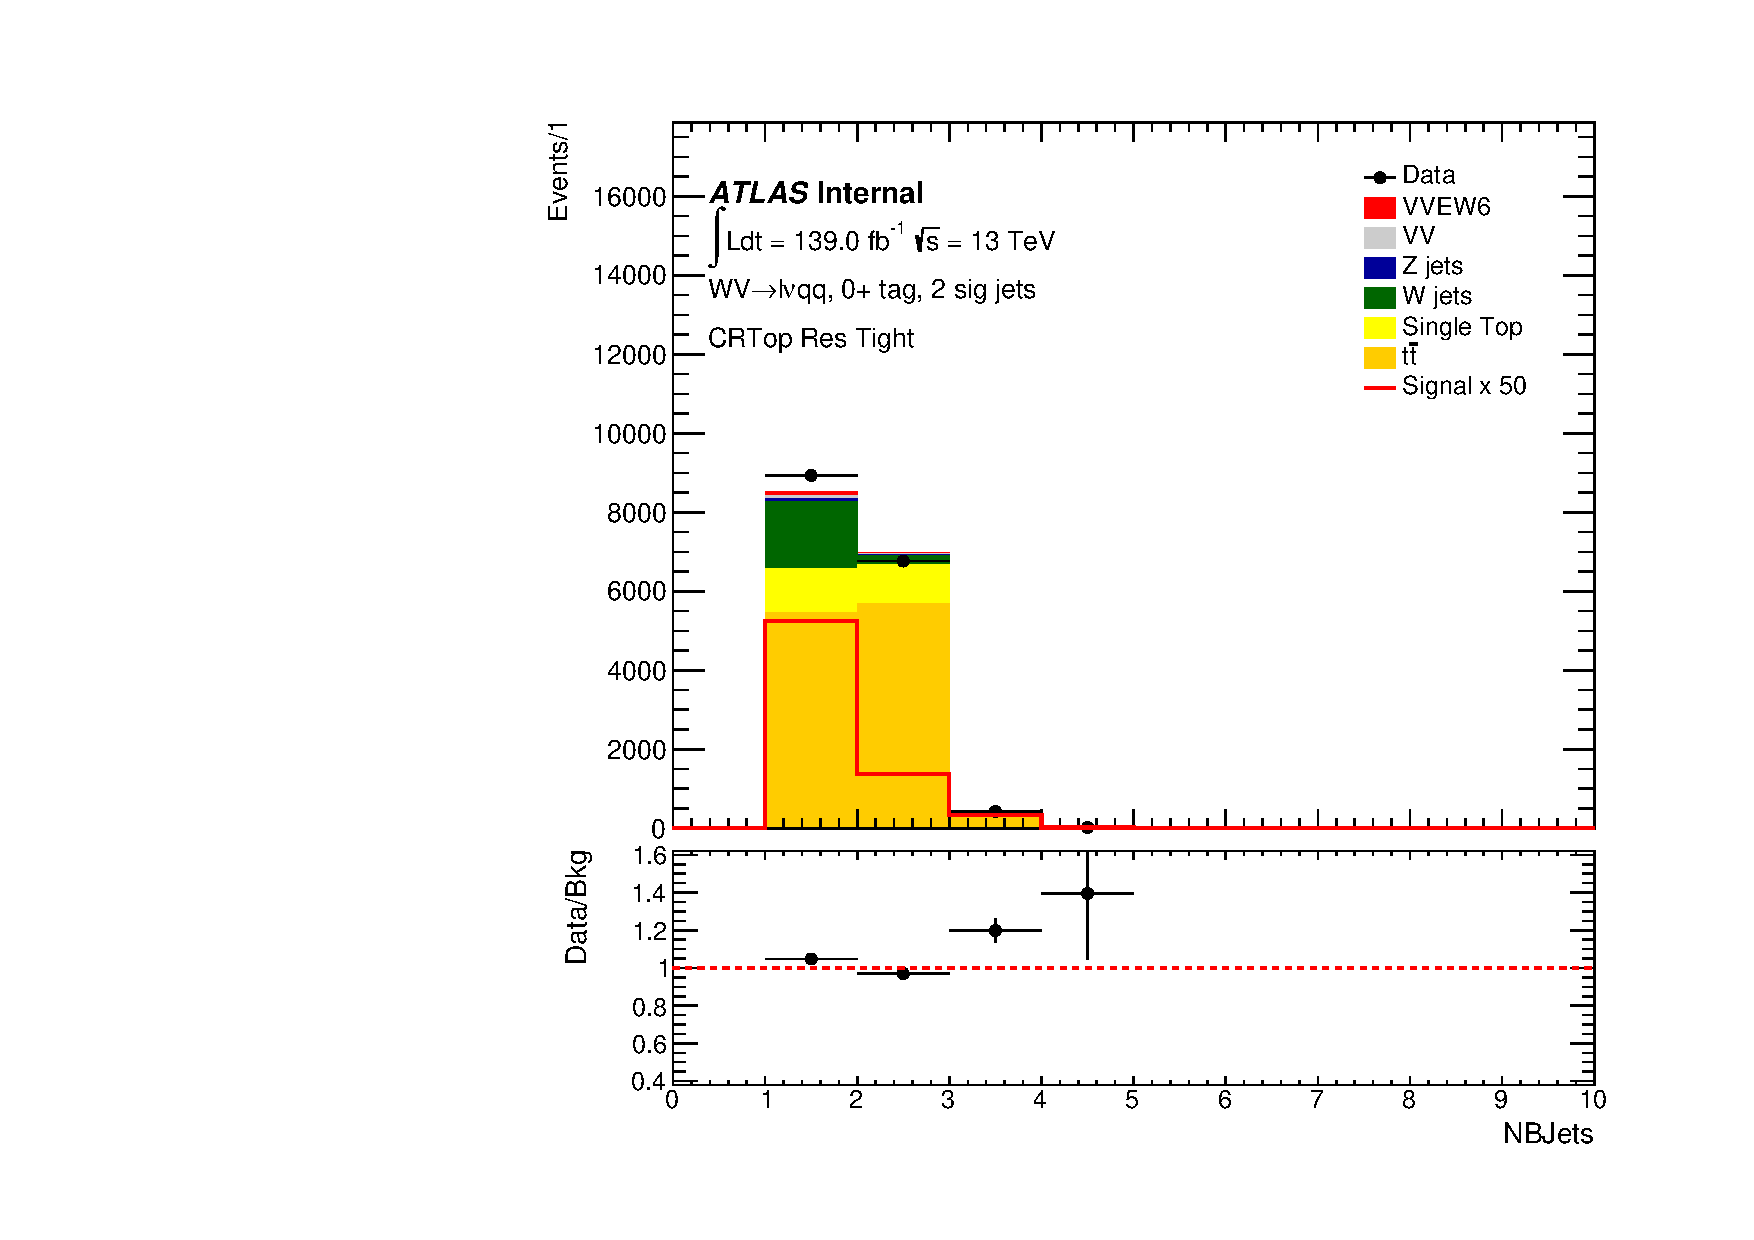
\includegraphics[width=\linewidth]{figures/CRPlots/CRTop_Res_Tight/stacked_plot_NBJets.pdf}
        \caption{Resolved TCR}
    \end{subfigure}
    \caption{$B$-jets multiplicity across various stages of event selection.}
    \label{fig:1lepNBjetsPresel}
\end{figure}

